%%%%%%%%%%%%%%%%%%%%%%%%%%%%%%%%%%%%%%%%%%%%%%%%%%%%%%%%%%%%%%%%%%%%%%%%%%%%%%%%%%
\begin{frame}[fragile]\frametitle{}
\begin{center}
{\Large Decision Tree - Heart Disease}

{\tiny (Ref: mlcourse.ai Assignment 3 – Open Machine Learning Course ) }
\end{center}

\end{frame}

%%%%%%%%%%%%%%%%%%%%%%%%%%%%%%%%%%%%%%%%%%%%%%%%%%%%%%%%%%
\begin{frame}[fragile]\frametitle{Problem Info}
Decision Tree for regression	
\begin{itemize}
\item Download data from https://github.com/Yorko/mlcourse.ai/blob/master/data/mlbootcamp5\_train.csv
\item Predict presence or absence of cardiovascular disease (CVD) using the patient examination results.

\end{itemize}
\end{frame}


%%%%%%%%%%%%%%%%%%%%%%%%%%%%%%%%%%%%%%%%%%%%%%%%%%%%%%%%%%
\begin{frame}[fragile]\frametitle{Read Data}	
\begin{lstlisting}
df = pd.read_csv('data/mlbootcamp5_train.csv', index_col='id', sep=',')
df.head()	 
\end{lstlisting}
\begin{center}
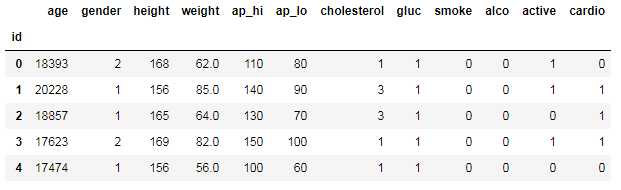
\includegraphics[width=0.8\linewidth,keepaspectratio]{dt21}
\end{center}
\end{frame}

%%%%%%%%%%%%%%%%%%%%%%%%%%%%%%%%%%%%%%%%%%%%%%%%%%%%%%%%%%
\begin{frame}[fragile]\frametitle{Transform Data}	
\begin{itemize}
\item Transform the features: create "age in years" (full age) and also create 3 binary features based on cholesterol and 3 more on gluc, where they are equal to 1, 2 or 3. 
\item This method is called dummy-encoding or One Hot Encoding (OHE). 
\item It is more convenient to use pandas.get\_dummmies.
\item There is no need to use the original features cholesterol and gluc after encoding.
\end{itemize}
\end{frame}

%%%%%%%%%%%%%%%%%%%%%%%%%%%%%%%%%%%%%%%%%%%%%%%%%%%%%%%%%%
\begin{frame}[fragile]\frametitle{Transform Data}	
\begin{lstlisting}
df['age_years'] = (df.age / 365.25).astype('int')
train_df = pd.get_dummies(df, columns=['cholesterol', 
                                       'gluc']).drop(['cardio'],
                                                     axis=1)
target = df.cardio
train_df.head()
\end{lstlisting}
\begin{center}
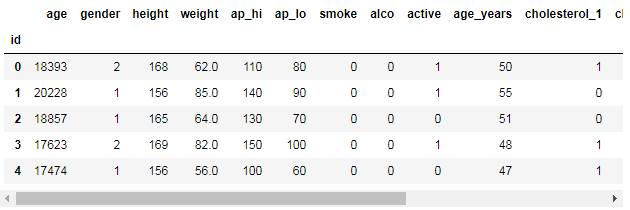
\includegraphics[width=0.8\linewidth,keepaspectratio]{dt22}
\end{center}
\end{frame}

%%%%%%%%%%%%%%%%%%%%%%%%%%%%%%%%%%%%%%%%%%%%%%%%%%%%%%%%%%
\begin{frame}[fragile]\frametitle{Split Data}	
Split data into train and holdout parts in the proportion of 7/3 using sklearn.model\_selection.train\_test\_split with random\_state=17.
\begin{lstlisting}
X_train, X_valid, y_train, y_valid = train_test_split(train_df.values, 
                                                      target.values,
                                                     test_size=.3, 
                                                      random_state=17)
\end{lstlisting}
\end{frame}

%%%%%%%%%%%%%%%%%%%%%%%%%%%%%%%%%%%%%%%%%%%%%%%%%%%%%%%%%%
\begin{frame}[fragile]\frametitle{Training Decision Tree}	
Split data into train and holdout parts in the proportion of 7/3 using sklearn.model\_selection.train\_test\_split with random\_state=17.
\begin{lstlisting}
clf = DecisionTreeClassifier(max_depth=5, random_state=17)

clf.fit(X_train, y_train)

export_graphviz(clf,out_file='tree.dot') 
\end{lstlisting}
\end{frame}

%%%%%%%%%%%%%%%%%%%%%%%%%%%%%%%%%%%%%%%%%%%%%%%%%%%%%%%%%%
\begin{frame}[fragile]\frametitle{Question 1}
What 3 features are used to make predictions in the created decision tree?	
\begin{itemize}
\item weight, height, gluc=3
\item smoke, age, gluc=3
\item age, weight, chol=3
\item age, ap\_hi, chol=3
\end{itemize}
Answer 4
\end{frame}

%%%%%%%%%%%%%%%%%%%%%%%%%%%%%%%%%%%%%%%%%%%%%%%%%%%%%%%%%%
\begin{frame}[fragile]\frametitle{Predictions}
Make predictions for holdout data (X\_valid, y\_valid) with the trained decision tree. Calculate accuracy.

\begin{lstlisting}
tree_pred_valid = tree.predict(X_valid) 
tree_acc_valid = accuracy_score(y_valid, tree_pred_valid)
tree_acc_valid
>>>
0.7212857142857143
\end{lstlisting}
\end{frame}


%%%%%%%%%%%%%%%%%%%%%%%%%%%%%%%%%%%%%%%%%%%%%%%%%%%%%%%%%%
\begin{frame}[fragile]\frametitle{Predictions}
\begin{itemize}
\item Set up the depth of the tree using cross-validation on the dataset (X\_train, y\_train) in order to increase quality of the model. 
\item Use GridSearchCV with 5 folds. Fix random\_state=17 and change  max\_depth from 2 to 10.
\end{itemize}
\end{frame}

%%%%%%%%%%%%%%%%%%%%%%%%%%%%%%%%%%%%%%%%%%%%%%%%%%%%%%%%%%
\begin{frame}[fragile]\frametitle{Predictions}
Make predictions for holdout data (X\_valid, y\_valid) with the trained decision tree. Calculate accuracy.

\begin{lstlisting}
tree_params = {'max_depth': list(range(2, 11))}

tree_grid = GridSearchCV(DecisionTreeClassifier(random_state=17), 
                         tree_params, cv=5, scoring='accuracy') 

tree_grid.fit(X_train, y_train)
\end{lstlisting}
\end{frame}


%%%%%%%%%%%%%%%%%%%%%%%%%%%%%%%%%%%%%%%%%%%%%%%%%%%%%%%%%%
\begin{frame}[fragile]\frametitle{Predictions}
Draw the plot to show how mean accuracy is changing in regards to max\_depth value on cross-validation.
\begin{lstlisting}
plt.plot(tree_params['max_depth'], 
         tree_grid.cv_results_['mean_test_score'])
plt.xlabel('Max depth')
plt.ylabel('Mean CV accuracy');
\end{lstlisting}
\begin{center}
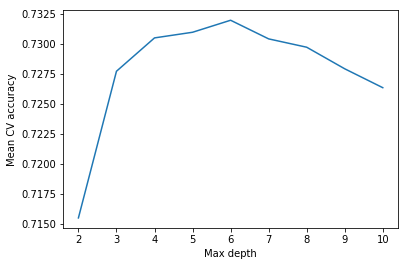
\includegraphics[width=0.5\linewidth,keepaspectratio]{dt23}
\end{center}
\end{frame}



%%%%%%%%%%%%%%%%%%%%%%%%%%%%%%%%%%%%%%%%%%%%%%%%%%%%%%%%%%
\begin{frame}[fragile]\frametitle{Predictions}
\begin{itemize}
\item Print the best value of max\_depth where the mean value of cross-validation quality metric reaches maximum. 
\item Also compute accuracy on holdout data. 
\item All these computations are possible to make using the trained instance of the class GridSearchCV.
\end{itemize}

\end{frame}

%%%%%%%%%%%%%%%%%%%%%%%%%%%%%%%%%%%%%%%%%%%%%%%%%%%%%%%%%%
\begin{frame}[fragile]\frametitle{Predictions}
\begin{lstlisting}
print("Best params:", tree_grid.best_params_)
print("Best cross validaton score", tree_grid.best_score_)
>>
Best params: {'max_depth': 6}
Best cross validaton score 0.7319591836734693

tuned_tree_acc_valid = accuracy_score(y_valid, 
                                      tree_grid.predict(X_valid))
tuned_tree_acc_valid
>>
0.7258095238095238

(tuned_tree_acc_valid / tree_acc_valid - 1) * 100
>>
0.6271869016966969

\end{lstlisting}
\end{frame}


%%%%%%%%%%%%%%%%%%%%%%%%%%%%%%%%%%%%%%%%%%%%%%%%%%%%%%%%%%
\begin{frame}[fragile]\frametitle{Question 2}
Is there a local maximum of accuracy on the built validation curve? 
Did GridSearchCV help to tune max\_depth so that there's been at least 1\% change in holdout accuracy? (check out the expression (acc2 - acc1) / acc1 * 100\%, where acc1 and acc2 are accuracies on holdout data before and after tuning max\_depth with GridSearchCV respectively)?

\begin{itemize}
\item yes, yes
\item yes, no
\item no, yes
\item no, no
\end{itemize}

Answer: 2
\end{frame}

%%%%%%%%%%%%%%%%%%%%%%%%%%%%%%%%%%%%%%%%%%%%%%%%%%%%%%%%%%
\begin{frame}[fragile]\frametitle{Question 3}
What binary feature is the most important for heart disease detection (it is placed in the root of the tree)?

\begin{itemize}
\item Systolic blood pressure from 160 to 180 (mmHg)
\item Gender male / female
\item Systolic blood pressure from 140 to 160 (mmHg) 
\item Age from 50 to 55 (years)
\item Smokes / doesn't smoke
\item Age from 60 to 65 (years)
\end{itemize}
\end{frame}

%%%%%%%%%%%%%%%%%%%%%%%%%%%%%%%%%%%%%%%%%%%%%%%%%%%%%%%%%%
\begin{frame}[fragile]\frametitle{Predictions}
\begin{lstlisting}
sub_df = pd.DataFrame(df.smoke.copy())
sub_df['male']  = df.gender - 1

sub_df['age_40_50'] = ((df.age_years >= 40) 
                       & (df.age_years < 50) ).astype('int')
sub_df['age_50_55'] = ((df.age_years >= 50) 
                       & (df.age_years < 55) ).astype('int')
sub_df['age_55_60'] = ((df.age_years >= 55) 
                       & (df.age_years < 60) ).astype('int')
sub_df['age_60_65'] = ((df.age_years >= 60) 
                       & (df.age_years < 65) ).astype('int')

sub_df['ap_hi_120_140'] = ((df.ap_hi >= 120) 
                           & (df.ap_hi < 140)).astype('int')
sub_df['ap_hi_140_160'] = ((df.ap_hi >= 140) 
                           & (df.ap_hi < 160)).astype('int')
sub_df['ap_hi_160_180'] = ((df.ap_hi >= 160) 
                           & (df.ap_hi < 180)).astype('int')

sub_df['chol=1'] = (df.cholesterol == 1).astype('int')
sub_df['chol=2'] = (df.cholesterol == 2).astype('int')
sub_df['chol=3'] = (df.cholesterol == 3).astype('int')
\end{lstlisting}
\end{frame}

%%%%%%%%%%%%%%%%%%%%%%%%%%%%%%%%%%%%%%%%%%%%%%%%%%%%%%%%%%
\begin{frame}[fragile]\frametitle{Predictions}
\begin{lstlisting}
sub_df.head()
\end{lstlisting}
\begin{center}
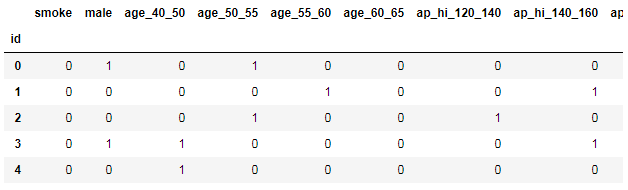
\includegraphics[width=\linewidth,keepaspectratio]{dt24}
\end{center}
\end{frame}

%%%%%%%%%%%%%%%%%%%%%%%%%%%%%%%%%%%%%%%%%%%%%%%%%%%%%%%%%%
\begin{frame}[fragile]\frametitle{Predictions}
\begin{lstlisting}
tree = DecisionTreeClassifier(max_depth=3, 
                              random_state=17).fit(sub_df, target)
							  print(df.columns)
export_graphviz(tree,out_file='newtree.dot') 
print(tree.feature_importances_)

>>
Index(['gender', 'smoke', 'cholesterol_1', 'cholesterol_2', 'cholesterol_3',
       'ap_hi_in_int_0', 'ap_hi_in_int_1', 'ap_hi_in_int_2', 'ap_hi_in_int_3',
       'age_in_int_0', 'age_in_int_1', 'age_in_int_2', 'age_in_int_3'],
      dtype='object')
[6.09602399e-04 1.68347891e-04 4.10705839e-05 1.75176127e-03
 1.48275116e-01 0.00000000e+00 7.57399191e-04 5.06561861e-01
 2.16891626e-01 8.72509796e-05 2.97702459e-05 4.48757380e-02
 7.99504559e-02]
\end{lstlisting}
\end{frame}
